\documentclass[a3paper]{article}
\usepackage[left=2mm,top=1cm,right=0mm,bottom=0mm]{geometry}
% \documentclass[border=0]{standalone}
\usepackage{tikz}
\usepackage{xcolor}
\definecolor{pGreen}{HTML}{006633}
\definecolor{sgbGreen1}{HTML}{66cc99}
\definecolor{sgbGreen2}{HTML}{ccffcc}

\definecolor{pRed}{HTML}{cc0033}
\definecolor{sgbRed}{HTML}{cc6688}
\definecolor{sgbRed2}{HTML}{FF99CC}

\definecolor{sgbGrey}{HTML}{333333}
\definecolor{sgbGrey2}{HTML}{996666}
\definecolor{sgbGrey3}{HTML}{999966}

\begin{document}
\pagecolor{sgbGrey3}
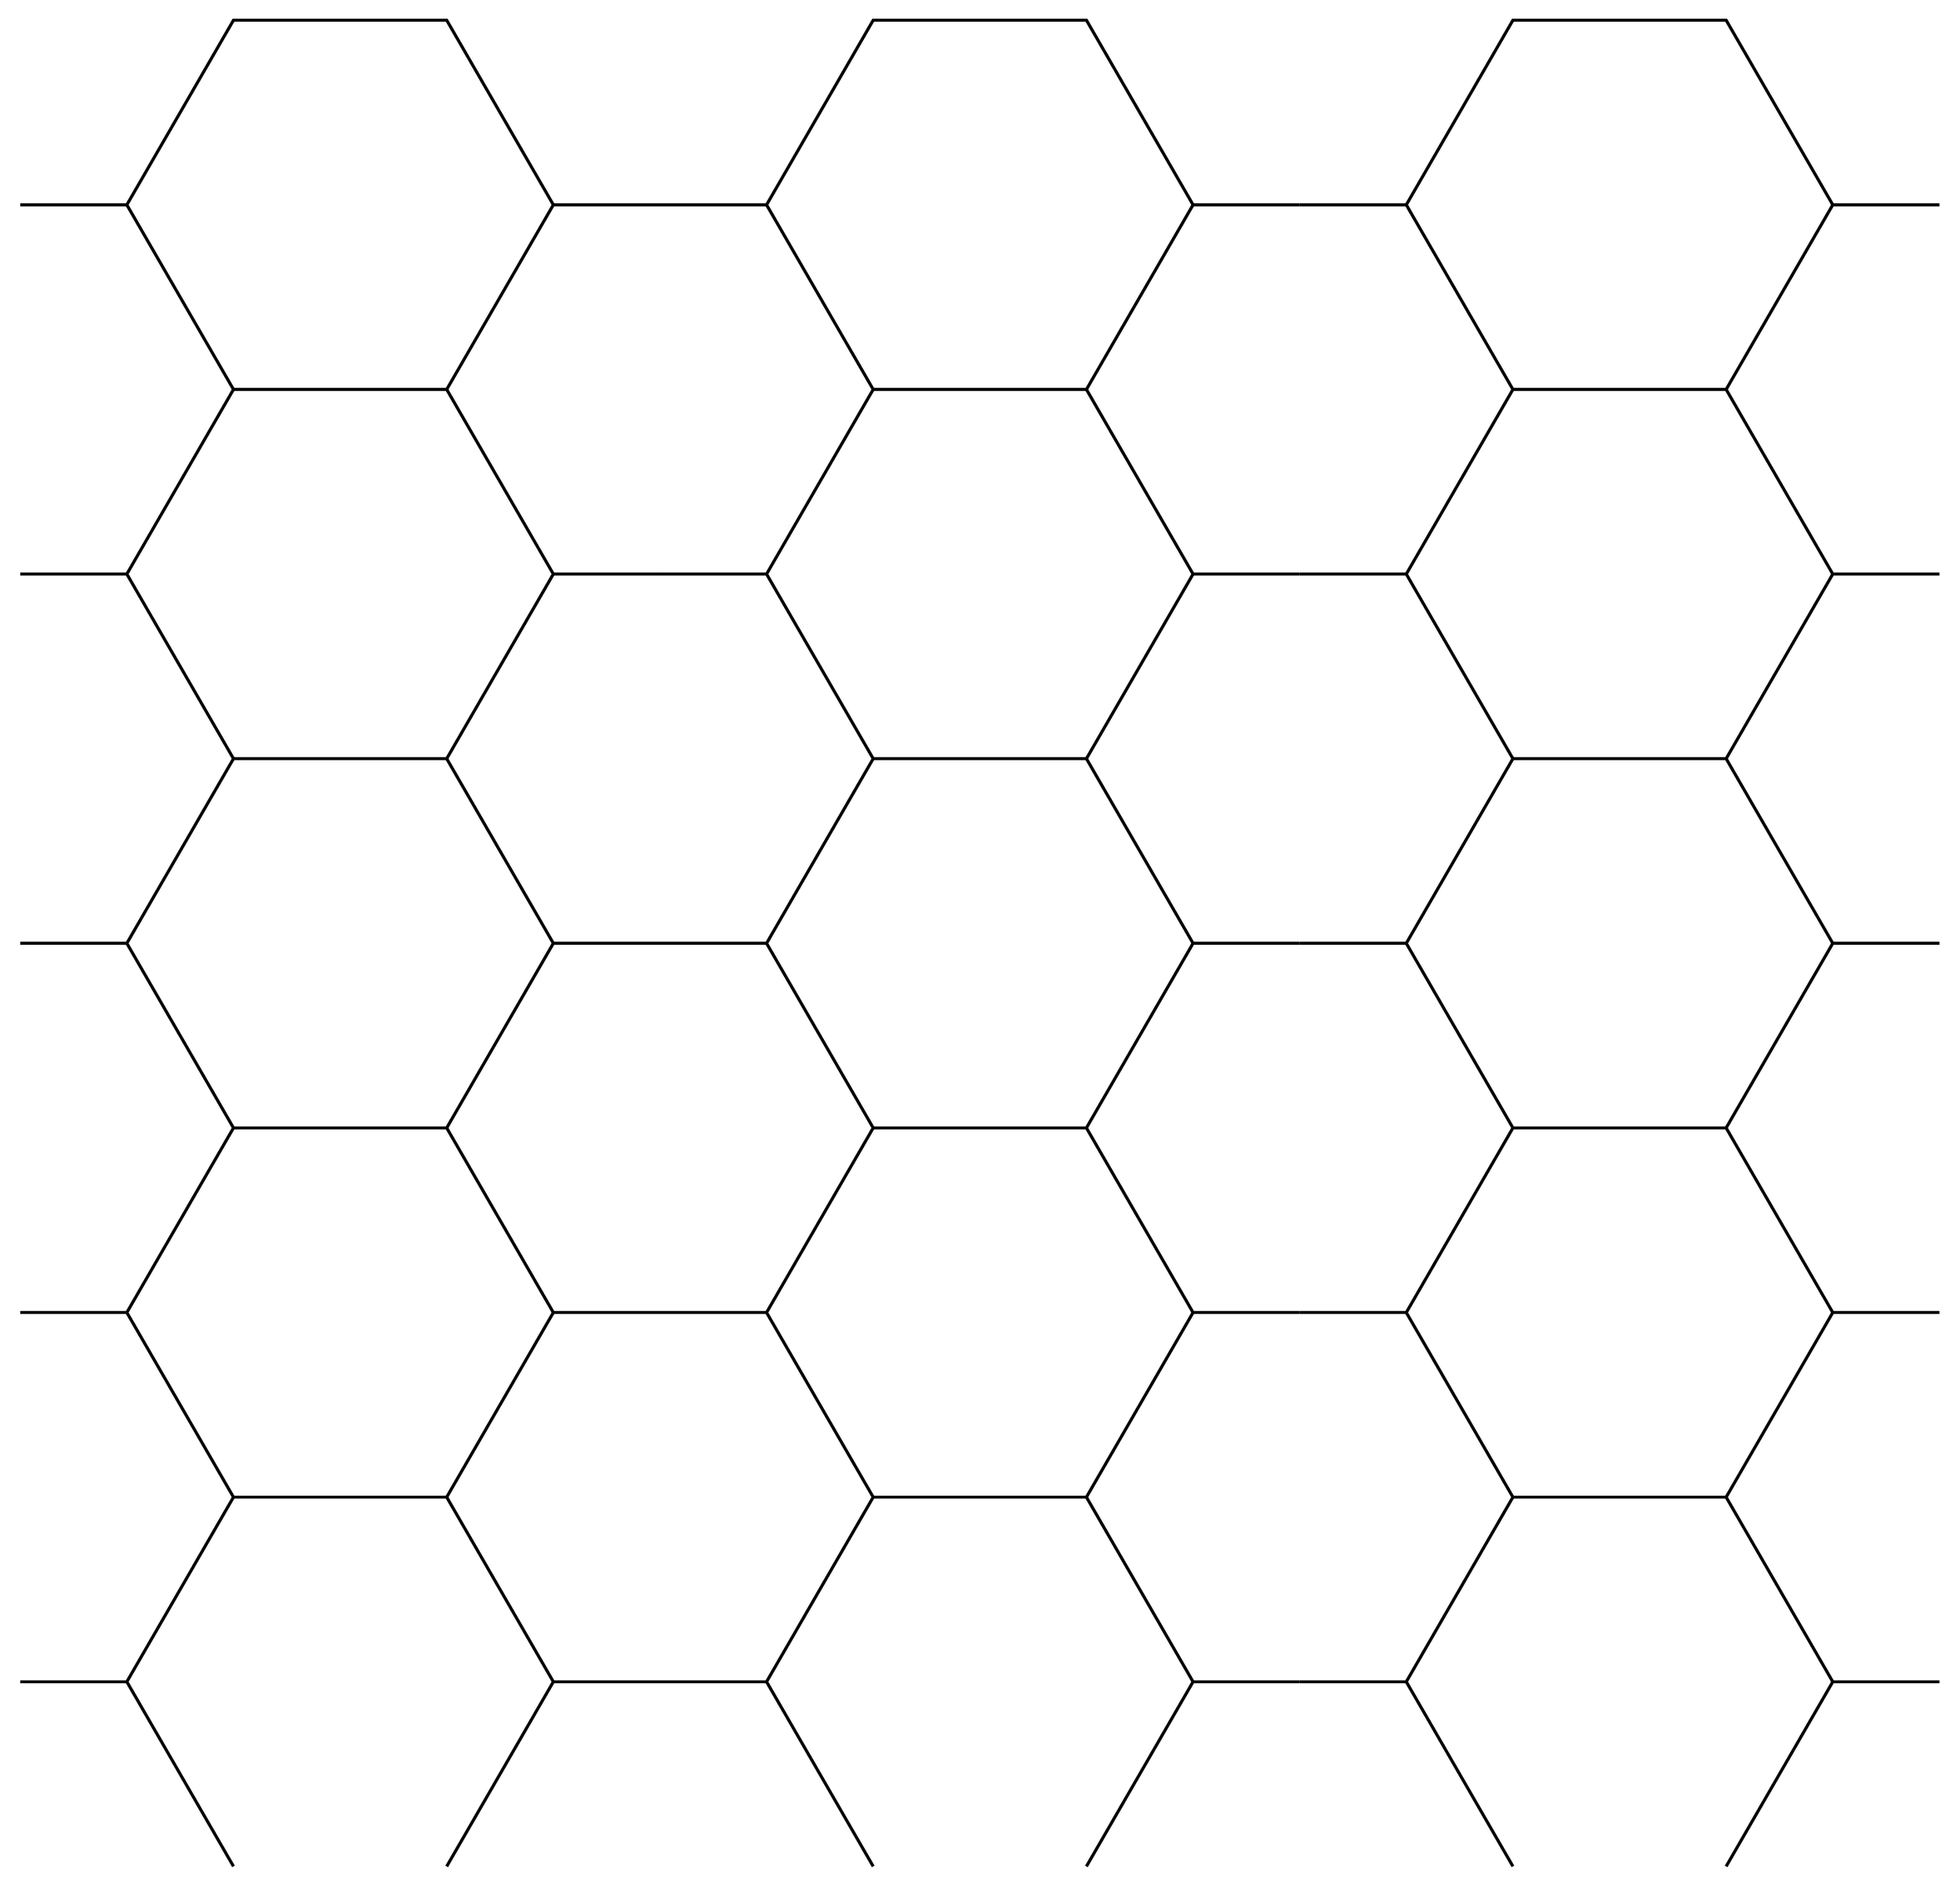
\begin{tikzpicture}
    \pgfmathsetmacro{\w}{4}
    \tikzset{cell/.pic={
        \draw[ultra thick] (0,0) -- (0:{\w/2}) --++ (60:\w) --++ (0:\w) --++ (-60:\w)--++(0:{\w/2});
        \draw[ultra thick] (0:{\w/2})--++(-60:\w);
        \draw[ultra thick] (0:{2.5*\w})--++(-120:\w); 
    }}
    \foreach \x in {0,1,2}{
        \foreach \y in {0,...,4}{
            \draw ({3*\w*\x},{2*\w*sin(60)*\y}) pic {cell};
        }
    }
\end{tikzpicture}
\end{document}

\foreach \row in {0,...,3}{
    \draw (0,{\row*sqrt(3)/2}) --++ (0:3);
    \draw (\row,0) --++ (60:4);
    \draw (\row,0) --++ (120:4);}